
%%% Uncomment for slide version
\documentclass[xcolor=dvipsnames]{beamer}
\setbeameroption{hide notes} % Only slides

%%% Uncomment for handout version
%\documentclass[handout]{beamer}
%\setbeameroption{show notes on second screen=right} % Both

\usepackage{enumitem}
\usepackage{listings}
\usepackage{adjustbox} % To incorporate code into Latex
\usepackage{multirow} % To merge multiple rows  in a table
\usepackage{soul} % To put in strikethrough text
\usepackage{array}
\usepackage{makecell}

\setbeamertemplate{note page}{\pagecolor{white}\insertnote}
\setbeamertemplate{footline}{}
\usetheme[progressbar=frametitle]{moloch}% modern fork of the metropolis theme
\setbeamercolor{background canvas}{bg=white}
\setbeamercolor{frametitle}{fg=black,bg=ProcessBlue!20}

\setbeamercolor{progress bar}{use=palette primary,fg=black,bg=black}
\setbeamercolor{note page}{bg=white} 
\setbeamertemplate{date}{}


\DeclareUnicodeCharacter{0313}{*************************************}

\setbeamertemplate{page number in head/foot}{}


\addtobeamertemplate{navigation symbols}{}{%
	\usebeamerfont{footline}%
	\usebeamercolor[fg]{footline}%
	\hspace{1em}%
	\insertframenumber/\inserttotalframenumber
}
\setbeamercolor{itemize item}{fg=black}
\setbeamercolor{itemize subitem}{fg=black}
\setbeamercolor{itemize subsubitem}{fg=black}

\newcommand\blfootnote[1]{%
	\begingroup
	\renewcommand\thefootnote{}\footnote{#1}%
	\addtocounter{footnote}{-1}%
	\endgroup
}

%%%%%%%%%%%%%%%%%%
%%%%%%%%%%%%%%%%%%
%%%%%%%%%%%%%%%%%%
%%%%%%%%%%%%%%%%%%
%%%%%%%%%%%%%%%%%%
%%%%%%%%%%%%%%%%%%
%%%%%%%%%%%%%%%%%%




\title{\Huge FRST302: Forest Genetics}
\author{\Large Interlude I}
\date{\today}

\begin{document}
	\maketitle

\begin{frame}
\frametitle{What is a p-value?}
\pause
\Large \textit{The probability of a particular observation under the null hypothesis}

\end{frame}


\begin{frame}
	\frametitle{Flipping Coins}
	Assume you're flipping a \textbf{fair} coin\\ \pause
	\vspace{10pt}
	This gives us the probability of flipping tails as $Pr(Tails)=0.5$\\ \pause
	\vspace{10pt}
	\textbf{Q:} If you flipped the coin 5 times, what is the probability of getting tails each time? \\ \pause
	\vspace{10pt}
	\textbf{A:} $Pr($5 tails out of 5 flips$) = 0.5^5$	
	

\end{frame}



\begin{frame}
	\frametitle{Flipping Coins}

	\textbf{Q:} If you flipped the coin 5 times, what is the probability that you got exactly two tails? \\ \pause	
	\vspace{10pt}
	\textbf{A:} HHTTT, HTHTT, HTTHT, HTTTH, THHTT, THTHT, THTTH, TTHHT, TTHTH, TTTHH\\
	\vspace{10pt}
	\textit{10 possible ways to get it } \\
	
	\vspace{10pt}
	\textit{From 5 coin flips there are 32 possible outcomes}* \\
	
	\vspace{10pt}
	\textbf{A:} $Pr($2 heads out of 5 flips$) = 10/32 = 0.3125$	

\blfootnote{Write them all down if you get really bored!!}

\end{frame}

\begin{frame}
		\frametitle{Flipping Coins}
	Here's the \textit{probability distribution} of flipping a fair coin 5 times \\
				
		\centering{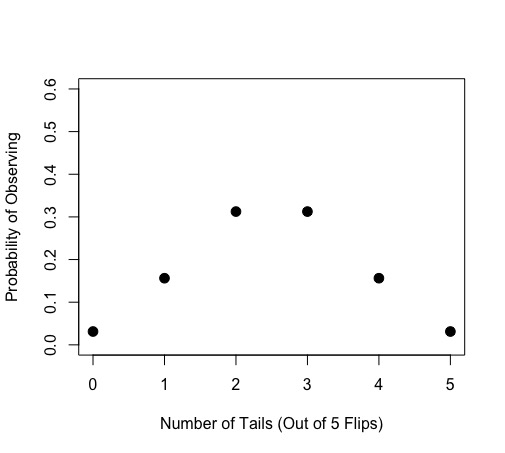
\includegraphics[keepaspectratio, width  = 0.5\textwidth]{img/5_flips}}\\
This is called the \textit{binomial} distribution
\blfootnote{Approximately 3\% of the time we would expect 0 tails in a set of 5 coin flips}
					
					
\end{frame}
\begin{frame}
			\centering{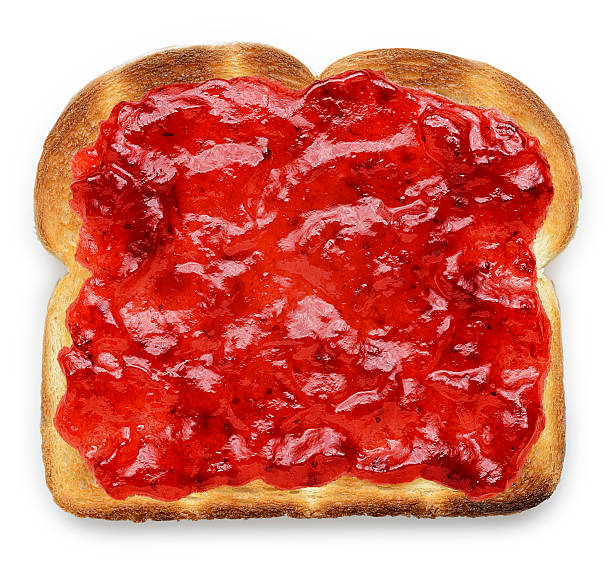
\includegraphics[keepaspectratio, width  = 0.7\textwidth]{img/jamtoast}}
\end{frame}



\begin{frame}
\frametitle{Jam Toast}
Is a dropped piece of toast equally likely to land jam side down, or jam side up?\\ 

\vspace{10pt}
Let's pretend that that we had 500 identical pieces of jam toast and we dropped them from the top of the FSC\\

\vspace{10pt}

What could we conclude about jam toast if in our experiment, it landed jam side down 100 times out of 500?\\ \pause

\vspace{10pt}

\textbf{Q:} What is the null hypothesis\\ \pause

\textbf{A:} That it's equally likely that dropped toast lands jam side or bread side up $Pr(Jam)=0.5$\\

	
	
	
\end{frame}






\begin{frame}
	\frametitle{Jam Toast}
	
Under this null hypothesis,\\
$Pr($100 jam-up toasts out of 500 drops$) =$\\
$ \binom{500}{100}0.5^{100}\times(1-0.5)^{500-100}  = 6.24 \times 10^{-44}$
	


\vspace{20pt}
This probability \textbf{is} the \textit{p}-value - \textit{the probabiity of observing 100 jam-up toasts out of 500 toast drops assuming that both outcomes are equally likely} \\
\pause
	
\vspace{10pt}
	
That we got such an unexpected result could lead us to reject the null hypothesis that 
	
	\blfootnote{Don't worry about the maths, that's just there to show you that there's a way to calculate it}
	
\end{frame}

\end{document}


%%%
\begin{columns}
	\begin{column}{0.5\textwidth}
	\end{column}
	\begin{column}{0.5\textwidth}
	\end{column}
\end{columns}


\begin{frame}
	\frametitle{Recap}
	
	
	\begin{itemize}
		\item[--] Introduction to genetic modification and genome editing
		\item[--] Methods of genetic modification and genome editing
		\item[--] Application of these in forest biology	
		
	\end{itemize}



\begin{frame}
	\frametitle{Flipping Coins}
	What if we flipped the coin 500 times?\\ \pause
	There are $3.27\times 10^{150}$ possible outcomes\\ \pause
	Here's the probability distribution:\\
	
	\centering{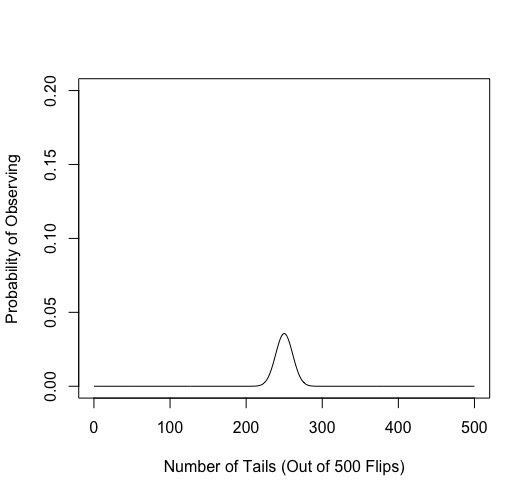
\includegraphics[keepaspectratio, width  = 0.6\textwidth]{img/500_flips}}\\
	
	
		\centering{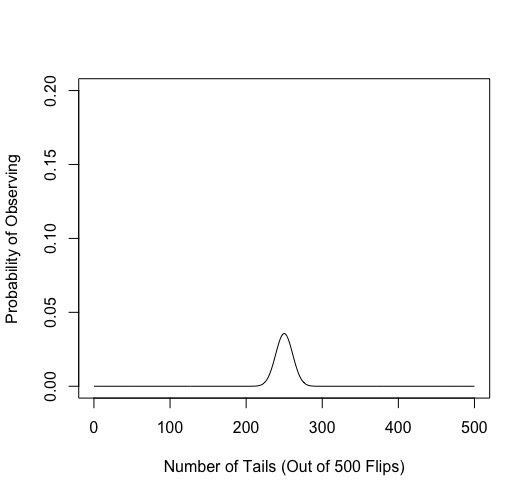
\includegraphics[keepaspectratio, width  = 0.6\textwidth]{img/500_flips}}\\
	
\end{frame}
